\chapter{Conception et analyse du système}
\chaptermark{Système}
\label{chapitre:systeme}

    \section{Introduction}

        Dans ce chapitre, nous allons réaliser les premières étapes de la conception du système de simulation. Dans un premier temps, nous allons réaliser une étude de l'existant afin de rendre compte des solutions permettant de simuler des environnements marins et sous-marins. Ensuite, nous allons établir les spécifications fonctionnelles de notre simulateur afin de définir les différentes fonctions que devra remplir notre système. Puis, nous allons élaborer les spécifications techniques de notre système, c’est-à-dire que nous allons déterminer les solutions techniques à employer afin de respecter le cahier des charges fonctionnelles. Enfin, nous seront en mesure de présenter une architecture logicielle pour notre simulateur, c'est-à-dire que nous allons présenter la manière dont vont s'agencer les différentes solutions techniques afin de produire le simulateur.

    \section{Etude de l'existant}

        La simulation de milieux marins est quelque chose de connu dans le domaine de la robotique, et il en existe aujourd'hui déjà de nombreux~\cite{Manhaes_2016, bingham19toward, MARS, Rock}. Ces simulateurs proposent tous un modèle de flottabilité pour les objets à simuler, ce qui permet de pouvoir définir à la fois des bateaux et des robots sous-marins. Cela permet donc de pouvoir simuler le comportement des \gls{ROV}s dans l'eau. Ils proposent ensuite tous leur lot de spécificités qui permettent d'avoir des éléments supplémentaires dans notre simulation.
        
        \textit{UUV Simulator}~\cite{Manhaes_2016} est probablement le plus connu d'entre eux. C'est un simulateur de \gls{ROV} comportant un certain nombre d'éléments d'environnements simulés, comme des mondes marins, du courant ou des ombilicaux par exemple. Il propose aussi la description d'un bon nombre de robots sous-marins commercialisés et la communauté active partage de nouveaux modèles régulièrement.
        
        \textit{Mars}~\cite{MARS} est un simulateur spécifique à des robots baptisés \textit{Mars}. Il permet de supporter plusieurs \gls{ROV}s et peut être commandé par \gls{ROS2} ou bien en utilisant des sockets TCP.
        
        \textit{Rock-Gazebo}~\cite{Rock} est un projet d'intégration de simulateur basé sur le moteur physique \gazebo{} et sur le framework\footnote{Infrastructure logicielle facilitant le développement logiciel} \textit{Robot Construction Kit}.
        
        Le simulateur \textit{VRX}~\cite{bingham19toward} est un projet open-source de robotique marine dont un simulateur a été implémenté sur la base de \gazebo{}. Il propose un ensemble d'environnement, de modèles et de plugin permettant la simulation de missions de vaisseaux de surface, avec notamment la possibilité de prendre en compte la présence de vagues et de vent à la surface.

        Ces simulateurs proposent tous des spécificités différentes et intéressantes. Cependant, notre application de simulation de \gls{ROV}s pour \forssea{} est assez contraignante. En effet, l'existence de composants spécifiques, comme la simulation de structures sous-marines transportables rendent l'adaptation de simulateurs existants trop difficile, d'autant qu'ils sont tous basés sur l'utilisation de la première version de \textit{ROS}. C'est pourquoi il est nécessaire de réaliser un simulateur propre à \forssea{}.

    \section{Spécifications fonctionnelles}
        \label{sec:spec_fonc}

        Le système à concevoir doit permettre de simuler \gls{ROV}s de la société \textsc{Forssea Robotics} dans un environnement sous-marin. Le simulateur doit respecter un certain nombre de spécifications fonctionnelles qui délimitent les exigences requises par le système. La \textsc{Figure}~\ref{figure:pieuvre} complétée par la \textsc{Table}~\ref{table:specs} présentent les exigences du système.

        \begin{figure}[!htb]
            \centering
            \begin{tikzpicture}[scale=0.7, every node/.style={ellipse, align=center, scale=0.7}]
                \node[draw,minimum height=40pt, minimum width=100pt, fill=VioletRed!70] (S) at (0, 0) {Simulateur};

                \node[draw,minimum height=40pt, minimum width=100pt, fill=Cerulean!80] (C0) at (0:5.5cm) {Robot};
                \node[draw,minimum height=40pt, minimum width=100pt, fill=Cerulean!80] (C1) at (72:2.8cm) {Environnement};
                \node[draw,minimum height=40pt, minimum width=100pt, fill=Cerulean!80] (C2) at (160:5cm) {Communication};
                \node[draw,minimum height=40pt, minimum width=100pt, fill=Cerulean!80] (C3) at (205:4.8cm) {Interface};
                \node[draw,minimum height=40pt, minimum width=100pt, fill=Cerulean!80] (C4) at (288:2.8cm) {Visualisation};

                \draw[blue!75, line width=0.8mm] (C0) -- (S) node[midway, fill=white]{\textbf{FP1}};
                \draw[blue!75, line width=0.8mm] (C1) -- (S) node[midway, fill=white]{\textbf{FP2}};
                \draw[orange!80, line width=0.8mm] (C2) -- (S) node[midway, fill=white]{\textbf{FC1}};
                \draw[orange!80, line width=0.8mm] (C3) -- (S) node[midway, fill=white]{\textbf{FC2}};
                \draw[orange!80, line width=0.8mm] (C4) -- (S) node[midway, fill=white]{\textbf{FC3}};
            \end{tikzpicture}
            \caption{Diagramme pieuvre du système}
            \label{figure:pieuvre}
        \end{figure}

        \begin{table}[!htb]
            \centering
            \begin{adjustbox}{max width=\textwidth}
                \begin{tabularx}{\textwidth}{|lX|}
                    \hline
                    \cellcolor{gray!25}\textbf{id} & \cellcolor{gray!25} \textbf{Fonction} \\
                    \hline \hline
                    \cellcolor{blue!30}\textbf{FP1}&\cellcolor{blue!25} Le système doit avoir un comportement proche du robot réel. \\
                    \hline
                    \cellcolor{gray!10}FP1.1& Le système doit avoir des dimensions semblables au robot réel. \\
                    \hline
                    \cellcolor{gray!10}FP1.2& Le système doit avoir des masses et des inerties semblables au robot réel. \\
                    \hline
                    \cellcolor{gray!10}FP1.3& Le système doit avoir les mêmes degrés de liberté que le robot réel. \\
                    \hline
                    \cellcolor{gray!10}FP1.5& Le système doit avoir les mêmes actionneurs que le robot réel. \\
                    \hline
                    \cellcolor{gray!10}FP1.4& Le système doit avoir les mêmes capteurs que le robot réel. \\
            
                    \hline \hline
            
                    \cellcolor{blue!30}\textbf{FP2}&\cellcolor{blue!25} Le système doit simuler l'environnement marin et sous-marin du robot \\
                    \hline
                    \cellcolor{gray!10}FP2.1& Le système doit simuler l'eau et les vagues. \\
                    \hline
                    \cellcolor{gray!10}FP2.2& Le système doit simuler des courants marins. \\
                    \hline
                    \cellcolor{gray!10}FP2.3& Le système doit simuler les ombilicaux reliant le \gls{ROV} au bateau. \\
                    \hline
                    \cellcolor{gray!10}FP2.4& Le système doit simuler les structures sous marines à transporter. \\
                    \hline
            
                    \hline \hline
            
                    \cellcolor{orange!40}\textbf{FC1} &\cellcolor{orange!30} Le système doit communiquer son état à l'utilisateur. \\
                    \hline
                    \cellcolor{gray!10}FC1.1& Le système doit communiquer l'état du robot à l'utilisateur. \\
                    \hline
                    \cellcolor{gray!10}FC1.2& Le système doit communiquer l'état de l'environnement à l'utilisateur.\\
                    \hline
            
                    \hline \hline
            
                    \cellcolor{orange!40}\textbf{FC2}&\cellcolor{orange!30} Le système doit être interfaçable avec le reste de l'implémentation logicielle. \\
                    \hline
                    \cellcolor{gray!10}FC2.1& Le système doit communiquer avec l'implémentation logicielle en \gls{ROS2}. \\
                    \hline
                    \cellcolor{gray!10}FC2.2& Le système doit être pilotable par les contrôleurs utilisés pour les robots réels. \\
                    \hline

                    \hline \hline
            
                    \cellcolor{orange!40}\textbf{FC3}&\cellcolor{orange!30} Le système doit être visualisable par l'utilisateur. \\
                    \hline
                    \cellcolor{gray!10}FC3.1& Le système doit pouvoir représenter les \gls{ROV}s dans leur environnement au cours de la simulation. \\
                    \hline
                    \cellcolor{gray!10}FC3.2& Le système doit fournir l'état des \gls{ROV}s et de l'environnement à l'utilisateur.  \\
                    \hline
                \end{tabularx}
            \end{adjustbox}
            \caption{Spécifications fonctionnelles du simulateur}
            \label{table:specs}
        \end{table}    

    \section{Spécifications techniques}

        Pour remplir les différentes spécifications fonctionnelles présentées dans la \textsc{Section}~\ref{sec:spec_fonc}, nous allons définir un certain nombre de spécifications techniques. Ces dernières vont proposer les outils et les différents critères permettant de remplir les exigences attendues.

        \subsection{Logiciel de simulation}

            L'étude de l'existant nous aura au moins permis de se rendre compte que \gazebo{}~\cite{Koenig-gazebo} est largement utilisé dans le domaine de la simulation sous-marine, mais aussi plus largement dans la simulation robotique. \gazebo{} est un logiciel de simulation multi-physique \textit{open-source}\footnote{Code communautaire ouvert libre de redistribution et d'accès}. Il est aujourd'hui développé par la communauté \textit{Open Robotics}\footnote{\url{https://www.openrobotics.org/}}.
            
            Il est possible de décrire précisément les robots, c'est-à-dire de décrire les couches visuelles, d'inerties et de collisions des robots afin de les simuler dans \gazebo{} en utilisant le langage \gls{SDF}\footnote{\url{http://sdformat.org/}}. Pour décrire le comportement de composants plus complexes comme des capteurs ou des actionneurs, un système de \textit{plugins} est disponible afin de laisser les développeurs ajouter des fonctionnalités à \gazebo{}. Ainsi la fonction principale \textbf{FP1} est remplie, car on est en mesure de simuler les robots avec des paramètres mécaniques proches du robot réel.

            De même, l'environnement est décrit à l'aide du langage \gls{SDF} et un système de \textit{plugins} permet d'interagir avec l'environnement de simulation afin d'ajouter des forces, des couples, ou bien des marqueurs visuels par exemple. Cela permet de remplir la fonction principale \textbf{FP2}.

            Ensuite, l'état du système est directement visualisable sur \gazebo{}. En effet, ce logiciel réalise la simulation et montre les robots évoluant dans leur environnement simulé, ce qui permet aussi de remplir une partie de la fonction contrainte \textbf{FC1}.

            Enfin, ce logiciel présente l'avantage de pouvoir communiquer avec \gls{ROS2}, ce qui satisfait la fonction contrainte \textbf{FC2}, en interfaçant le simulateur avec le reste de l'implémentation logicielle des robots.

        \subsection{Ignition Libraries}

            \textit{Ignition Libraries}\footnote{\url{https://ignitionrobotics.org/libs}} est un ensemble de libraries permettant de faciliter le développement robotique. Deux libraries permettent de compléter la fonction contrainte \textbf{FC1} : \textit{Ignition-Transport} et \textit{Ignition-Msgs}. Elles permettent de faire communiquer deux parties de codes ensemble grâce à un système de messagerie basée sur l'utilisation de la bibliothèque \textit{ProtocolBuffer} développée par \textit{Google}\footnote{\url{https://developers.google.com/protocol-buffers}}. C'est le même système de communication qui est utilisé par \gls{ROS2} et \gazebo{}. Ce système de communication présente l'avantage de diviser le code en n\oe uds pouvant s'exécuter en parallèle et communiquant ensemble par ces librairies, mais aussi de pouvoir récupérer l'état du simulateur par la lecture des messages transitant sur le réseau \textit{Ignition-Transport}. Ainsi on peut précisément savoir ce qu'il se passe dans le simulateur à chaque instant.

        \subsection{ROS2 Control}

            Pour respecter la fonction contrainte \textbf{FC2}, le simulateur doit s'interfacer avec le reste de l'implémentation logicielle, il est donc nécessaire de définir une architecture logicielle permettant de communiquer à la fois avec les \gls{ROV}s réels et simulés. \textit{ROS2 Control}~\cite{ros_control} est un framework permettant de faire communiquer des contrôleurs et des drivers ensemble. Le principal avantage est qu'il est temps-réel, c'est-à-dire que les données des capteurs sont accessible instantanément par les contrôleurs, les actionneurs ont aussi instantanément accès aux commandes, et enfin on peut changer de manière consistante de contrôleur, sans temps mort durant lesquels le robot ne serait pas commandé.

            \begin{figure}[!htb]
                \centering
                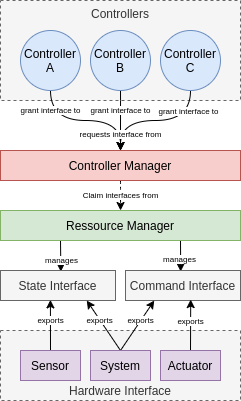
\includegraphics{build/diagrams/ros2_control.pdf}
                \caption{Architecture logicielle avec \textit{ROS2 Control}}
                \label{fig:ros2_control}
            \end{figure}

            La \textsc{Figure}~\ref{fig:ros2_control} nous montre l'architecture logicielle de \textit{ROS2 Control}. Ce framework va instancier un \textit{Controller Manager} qui va s'occuper de charger les contrôleurs qui seront utilisés dans le robot, des \textit{Hardware Interface} qui sont les interfaces qui vont communiquer avec les composants et un \textit{Ressource Manager} qui va faire transiter les données entre les contrôleurs et les composants. L'\textit{Hardware Interface} peut avoir pour rôle de communiquer avec les composants réels, où avec les composants simulés. L'idée est de créer une \textit{Hardware Interface} pour la simulation proposant les mêmes interfaces que celle implémentée pour les composants réels. Ainsi on peut utiliser les mêmes algorithmes de contrôle de manière totalement transparente pour commander le robot réel ou le simulateur et la fonction contrainte \textbf{FC2} est remplie.

        \subsection{Architecture Logicielle}

            En rassemblant ce qui a pu être présenté dans ce chapitre, on peut proposer l'architecture logicielle présentée sur la \textsc{Figure}~\ref{fig:architecture_logicielle} pour ce simulateur.
            
            Ce système nécessite donc dans un premier la description pour \gazebo{} d'un monde de simulation sous-marin ainsi que la description des \gls{ROV}s dans un premier temps afin de pouvoir simuler les robots. Puis vient l'implémentation de \textit{plugins} \gazebo{} et d'\textit{Hardware Interface} pour interagir et contrôler ces robots, qui communique ensemble par via les librairies \textit{ignition}.
            
            \begin{figure}[!htb]
                \centering
                \includegraphics[]{build/diagrams/architecture_logicielle.pdf}
                \caption{Architecture logicielle du simulateur}
                \label{fig:architecture_logicielle}
            \end{figure}

    \section{Conclusion}

        En conclusion, nous avons défini dans ce chapitre les exigences attendues pour ce simulateur. Elles nous ont permis de choisir des solutions techniques adaptées à la réalisation de ce système et nous avons donc pu proposer une architecture logicielle à mettre en place pour simuler correctement les \gls{ROV}s de \textit{Forssea Robotics}. Nous allons donc pouvoir commencer le développement de ce système en utilisant les outils mis en place dans ce chapitre.
        